\documentclass[a0,portrait]{a0poster}
%%%Load packages
\usepackage{multicol} 			%3-column layout
\usepackage[left=6cm,right=2cm,bottom=0cm,top=0cm]{geometry}			%Reset margins
\usepackage[T1]{fontenc}			%Need for gtamac fonts
\usepackage{textcomp}
\usepackage{mathpazo}			%Load palatino font & pazo math
\usepackage{color}				%Needed for colour boxes & coloured text
\usepackage{amsmath}


%%%Define colours and lengths
\definecolor{headingcol}{rgb}{1,1,1}		%Colour of main title
\definecolor{fillcol}{rgb}{1.0,1.0,1}			%Fill-colour of box
\definecolor{boxcol}{rgb}{0.6,0,0}		%Edge-colour of box and top banner
\definecolor{author}{rgb}{0.9, 0.9, 0.9}
\fboxsep=1cm							%Padding between box and text
\fboxrule=2mm							%Width of box outline
\renewcommand{\rmdefault}{ppl}			%Reset serif to Palatino
\setlength{\columnsep}{2cm}				%Set spacing between columns
%Uncomment for lines as column separators:
%\setlength{\columnseprule}{1pt}


%%%Format title
\makeatletter							%Needed to include code in main file
\renewcommand\@maketitle{%
\null									%Sets position marker
{
\vspace{2cm}
\color{headingcol}\sffamily\huge\bf		%Set title font and colour
\@title \par}%
\vskip 0.6em%
{
\color{author}\sffamily\large\bf				%Set author font and colour
\lineskip .5em%
\begin{tabular}[t]{l}%
\@author
\end{tabular}\par}%
\vskip 1cm
\par
}
\makeatother

\newsavebox\envbox 					%Define name for boxes used

%%%Define "Section" environment for framed boxes
%%%Usage: \begin{Section}{Name} blah blah blah \end{Section}
\newenvironment{Section}[1]				%Environment takes one argument
%%%Opening
{
\par 
\flushleft
\colorbox{boxcol}{% 						%Draws solid colour box around title
\sffamily\large\bf\color{headingcol}> \color{white} #1%Typesets section name
\hspace{0.5cm}}
\par\nobreak 
\nointerlineskip 						%Fits title snugly above box (no gap)
\setlength\parskip{-1pt}					%Even snugger
\begin{lrbox}\envbox						%Opens box environment
\begin{minipage}{0.95\columnwidth}		%Opens minipage environment for section contents
}
%%%Closing
{\par
\end{minipage}\end{lrbox}				%Close minipage and box
\fcolorbox{boxcol}{fillcol}{\usebox\envbox}	%Draw box with contents frame colour: boxcol, fill colour: fillcol
\vspace{1cm}							%Add spacing below box
} 
\newenvironment{Section2}[1]				%Environment takes one argument
%%%Opening
{
\par 
\flushleft
\colorbox{boxcol}{% 						%Draws solid colour box around title
\sffamily\large\bf\color{headingcol}> \color{white} #1%Typesets section name
\hspace{0.5cm}}
\par\nobreak 
\nointerlineskip 						%Fits title snugly above box (no gap)
\setlength\parskip{-1pt}					%Even snugger
\begin{lrbox}\envbox						%Opens box environment
    \begin{minipage}{1.9\columnwidth}		%Opens minipage environment for section contents
}
%%%Closing
{\par
\end{minipage}\end{lrbox}				%Close minipage and box
\fcolorbox{boxcol}{fillcol}{\usebox\envbox}	%Draw box with contents frame colour: boxcol, fill colour: fillcol
\vspace{1cm}							%Add spacing below box
} 
\usepackage{physics}
\usepackage{graphicx}
\graphicspath{ {images/} }
\usepackage{caption}

\title{Understanding Dissipative Control of Quantum Dynamics from Biased Trajectory Ensembles}

\author{Fergus Barratt}

\begin{document}

\hspace{-4.1cm}								%Align with edge of page, not margin
\colorbox{boxcol}{							%Coloured banner across top
\begin{minipage}{1189mm}					%Minipage for title contents
%\vspace{-13cm}							%Shift up over header image
\maketitle
\end{minipage}}
\vspace{1cm}

\begin{multicols}{3}							%Use 3-column layout
\raggedcolumns							%Don't stretch contents vertically

%%%Column1
\begin{Section}{Introduction}
\begin{itemize}
    \item The technological potential of quantum systems is due to the exponential scaling of the tensor product state space.
    \item Environmental decoupling represents a challenge to effective use of quantum technology.
    \item Tools from classical statistical mechanics can be used to quantify changes of dynamical behaviour in a range of systems.
    \item In particular, the methods of \emph{Biased Trajectory Ensembles} can be connected to dissipation in quantum systems. 
    \item We plan to study the transition from the presence of usable quantum resources (i.e. entanglement) to their absence.
\end{itemize}
\end{Section}

\begin{Section}{Keldysh Theory}
\begin{itemize}
    \item In the equilibrium formalism of quantum field theory, we rely on the adiabatic switching on and off of interactions bringing the system back into its ground state when evolved $t=-\infty \rightarrow t=\infty$
    \item Clearly not true in the non-equilibrium case
    \item Suggestion: evolve the state forward in time $(t=-\infty \rightarrow \infty)$, then rewind $t=\infty \rightarrow -\infty$: fig. \ref{fig:keldysh}
    \item Convenient to separate fields on forward and backwards contours ($\phi^+, \phi^-$)
    \item Constructing the path integral in usual way, there is a redundancy in the Green's Function description. 
    \item Defining
    \begin{equation}
        \phi^q = \phi^+ - \phi^- \qquad \phi^{cl} = \phi^+-\phi^-
    \end{equation}
    \item leads to Green's Functions with one component always 0
    \begin{align}
        \ev{\phi^q(t) \phi^q(t')} &= 0  \quad \ev{\phi^{cl}(t)\phi^{cl}(t')} = iG^K(t, t') \\
        \quad \ev{\phi^{cl}(t)\phi^{q}(t')} =& iG^R(t, t') \quad \ev{\phi^q(t)\phi^{cl(t')}} = iG^A(t, t')
    \end{align}
    \item Introducing a bath of oscillators interacting with system degrees of freedom, and integrating out the bath degrees of freedom, and expanding to first order in the quantum fields we can generate effective langevin descriptions of quantum dynamics.
    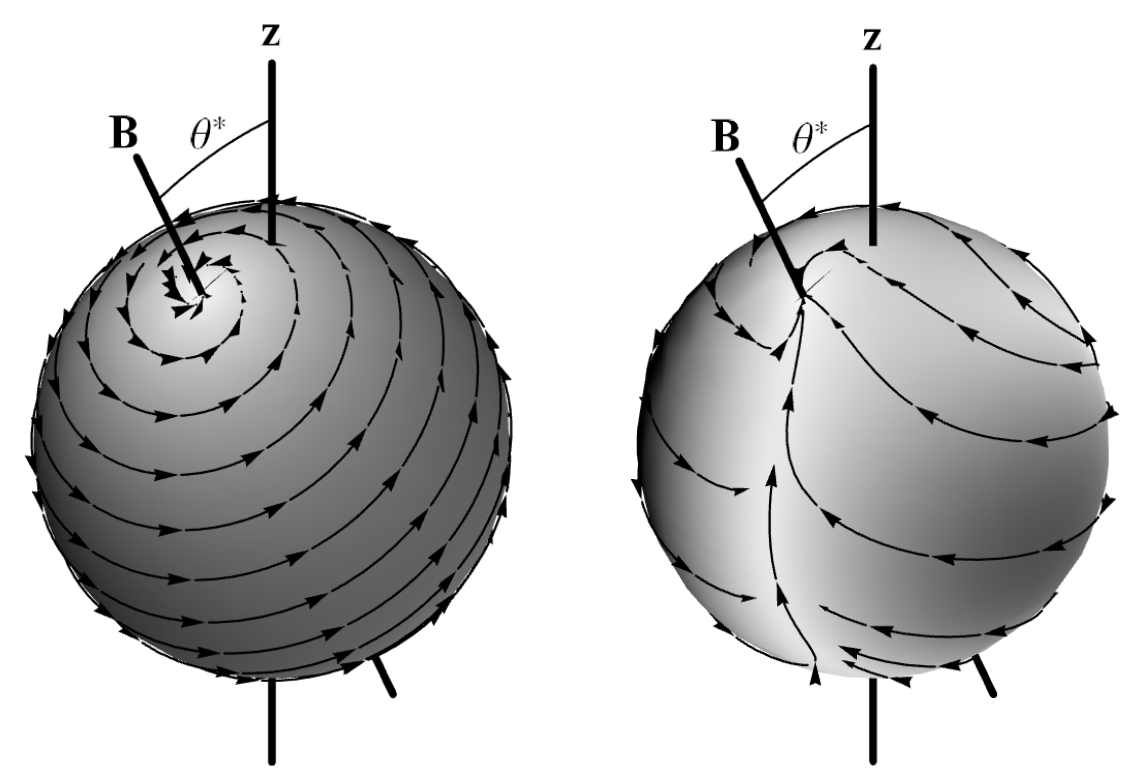
\includegraphics[width=\linewidth]{spins1}
\end{itemize}

\end{Section}

\begin{Section}{References}
    \bibliography{ref}{}
    \bibliographystyle{plain}
\end{Section}
\columnbreak

%%%Column 2
\begin{Section}{Matrix Product States}

    \hspace{1.5cm}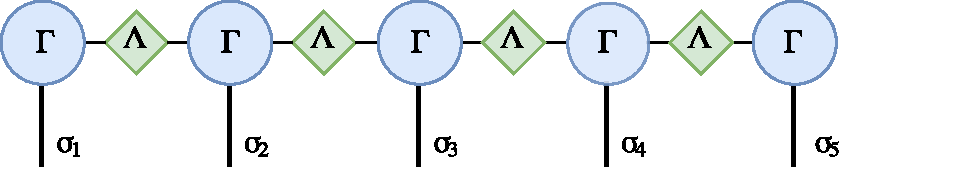
\includegraphics[width=\linewidth]{mps}
\captionof{figure}{Open Boundary Condition MPS in $\Gamma\Lambda$ notation}

\begin{itemize}
    \item DMRG constitutes the state of the art for the study of one dimensional quantum lattices.  
The study of the effectiveness of the DMRG algorithm leads naturally to the concept of Matrix Product States(MPS)

    \item The dimension of the product Hilbert space of a spin chain grows exponentially in its length ($\order{d^L}$ where d is the local Hilbert space dimension).
    This presents a problem for direct numerical methods. 

    \item However, by an entanglement argument \cite{Orus2014}, we can see that the interesting corner of the total Hilbert space is very small compared to the total space, and in fact this subspace permits an effective numerical description in terms of Matrix Product States.

    \item An arbitrary quantum state can be written
\begin{equation}
    \ket{\psi} = \sum_{\sigma_1, \ldots, \sigma_L} C_{\sigma_1, \ldots, \sigma_L} \ket{\sigma_1, \ldots, \sigma_L},\label{eq:quantum_state}
\end{equation}
Where $\ket{\sigma_i}$ is the local basis of the $ith$ space.

    \item Via an iterated Singular Value Decomposition (SVD) of the tensor reshaped into a matrix, we can express eq.\ref{eq:quantum_state} exactly as
    \begin{equation}
        \ket{\psi} = \sum_{\sigma_1, \ldots, \sigma_L} \Gamma^{\sigma_1}\Lambda_1 \ldots \Lambda_{L-1}\Gamma^{\sigma_L} \ket{\sigma_1, \ldots, \sigma_L }\label{eq:orus_mps}
    \end{equation}
    Where $\Gamma^{\sigma_i}$ denotes an indexed set of matrices, and  $\Lambda_i$ represents the singular values in the ith step of the decomposition.

\item The index structure of the $\Gamma$ matrices in each of these (exact) expressions goes $(1\times d), (d \times d^2), \ldots (d^2 \times d), (d\times 1)$ i.e. the largest matrix size grows exponentially with the length of the chain L.

\vspace{1cm}
\hspace{-1cm}
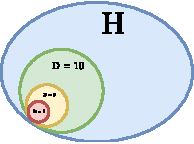
\includegraphics[ width=\linewidth]{D}
\captionof{figure}{Size of subset of Hilbert space $H$ with bond dimension $D$ grows with $D$}
\vspace{1cm}

\item Important corner of Hilbert space is spanned by Matrix Product states of form \ref{eq:orus_mps}, with all but $D$ of the singular values on each site set to zero (where $D$ is small) 
\end{itemize}
\end{Section}

\columnbreak

%%%Column 3

\begin{Section}{Trajectory Ensembles}
    \begin{itemize}
        \item By analogy to the ensembles of microstates of equilibrium statistical mechanics, in the study of glass forming systems (and elsewhere) ensembles of system trajectories have been studied~\cite{Garrahan2009}.
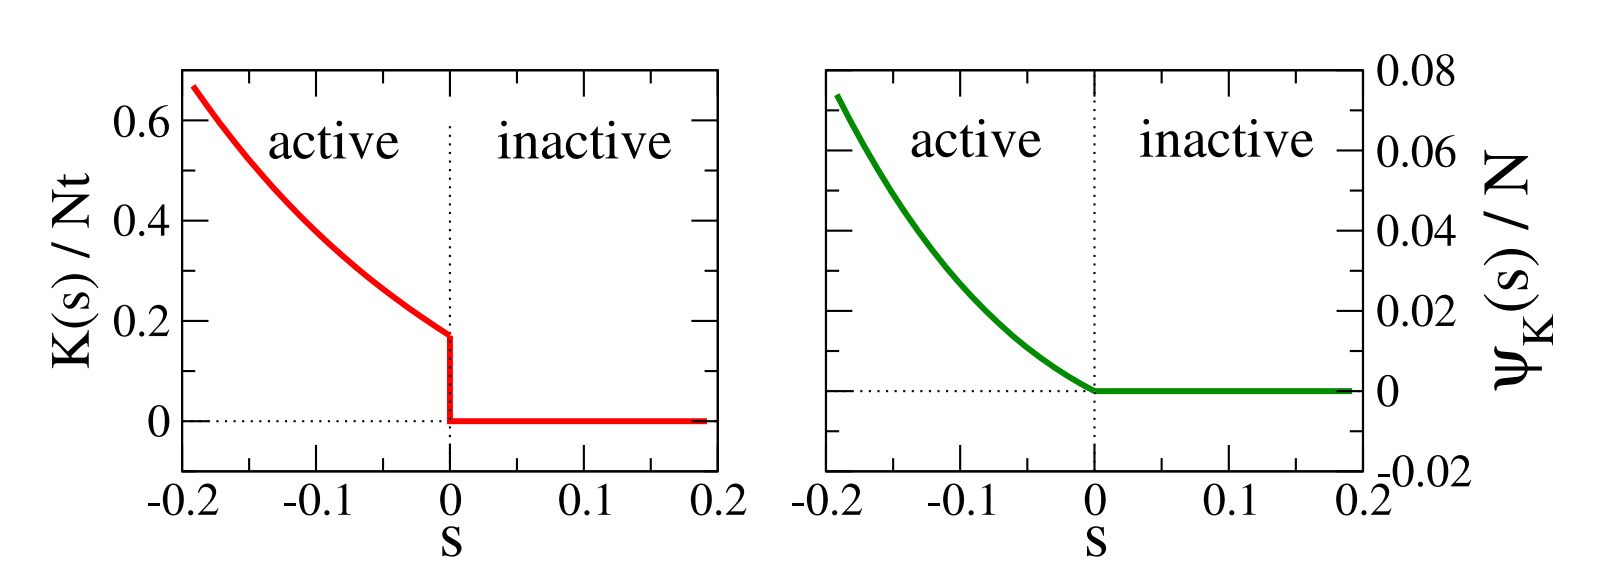
\includegraphics[width=\linewidth]{dyn_trans}
\captionof{figure}{Dynamical phase transition in a kinetically constrained model. $\mathcal{K}(s)$ is the first derivative of $\psi_K(s)$ the dynamical free energy\cite{Garrahan2007}}

\item Starting from Markovian dynamics, the trajectories are biased (as in the canonical ensemble) by the value of some time extensive observable on that trajectory.

\item At the level of the master equation, this corresponds to a deformation of the operator $\mathbb{W} \rightarrow \mathbb{W}_A$ in the vector form (s is a biasing field, the analogue of $\beta$ the inverse temperature)
\begin{equation}
    \pdv{\vec{P}_A}{t} = \mathbb{W}_A(s) \vec{P}_A,
\end{equation}
and from there for the dynamical analogue of the partition function
\begin{equation}
    \mathcal{Z}_A(s, t) \sim e^{t \psi_A(s)}
\end{equation}
where $\psi_A(s)$ is the largest eigenvalue of the matrix $\mathbb{W}_A(s)$ and the \emph{dynamical free energy}.
\item Singular values in the dynamical free energy signal \emph{dynamical phase transitions} from between regions of qualitatively different dynamical behaviour i.e. transition to chaos, jamming in glasses.
\item An example of a class of systems for which there are results on dynamical phase transitions are \emph{kinetically constrained models} (KCMS) of glass formers (\ref{fig:KCM})

\end{itemize}
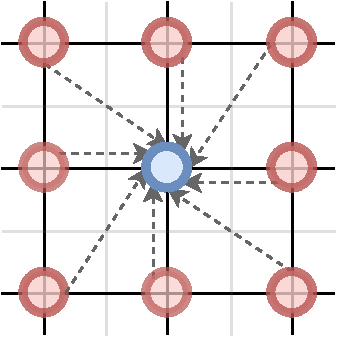
\includegraphics[width=\linewidth]{kcm}
\captionof{figure}{Schematic of site of Kinetically Constrained Model. Site $i$ (blue) transitions from $n_i \rightarrow 1-n_i$ with rate $W(n_i \rightarrow 1-n_i) = C(\{n_j\}) \frac{e^{\beta(n_i-1)}}{1+e^{-\beta}}$, where $C(\{n_j\})$ is a function only of the values of sites $n_j$ (red)} \label{fig:KCM}
\end{Section}
%\bibliographystyle{plain}
%\bibliography{halobib}

\end{multicols}
\begin{figure}[h]
    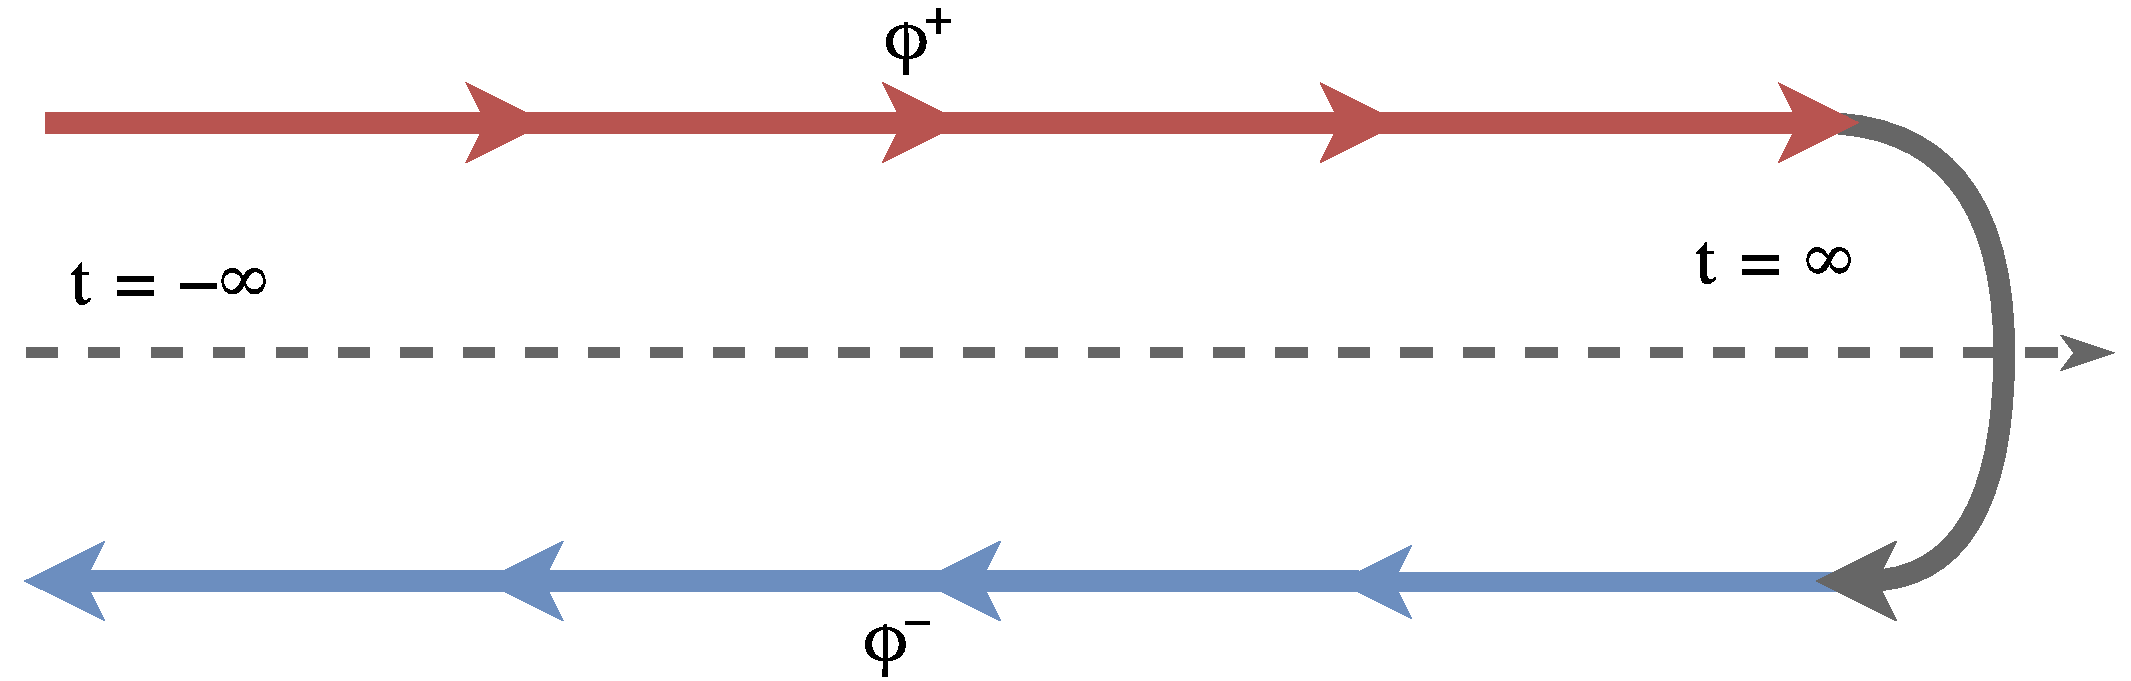
\includegraphics[width=\linewidth]{keldysh}
    \caption{Keldysh closed time contour}\label{fig:keldysh}
\end{figure}
\end{document}
